\documentclass[11pt]{article}

\usepackage{amsmath}
\usepackage[margin=0.68in]{geometry}
\usepackage{booktabs}
\usepackage{enumitem}
\usepackage{fancyhdr}
\usepackage{graphicx}
\usepackage[table]{xcolor}
\usepackage[hidelinks]{hyperref}
\usepackage{listings}
\usepackage{microtype}
\usepackage{tabularx}
\usepackage{titlesec}
\graphicspath{{docs/lessons/assets/}{../assets/}}

\definecolor{Ink}{gray}{0}
\definecolor{CodeGray}{gray}{0.96}
\hypersetup
{
    pdftitle={ADK Lesson 028: Synthetic Channel Assessment},
    pdfauthor={Kevin Shanahan},
    pdfsubject={Deterministic redundant observations, age, transactional updates, and inert LED evidence},
    pdflang={en-US}
}
\pagestyle{fancy}
\fancyhf{}
\lhead{\textsc{ADK Lesson 028}}
\rhead{Synthetic Channel Assessment}
\cfoot{\thepage}
\setlength{\headheight}{14pt}
\setlength{\parindent}{0pt}
\setlength{\parskip}{5pt}
\setlist{nosep,leftmargin=1.45em}
\titleformat{\section}{\Large\bfseries\color{Ink}}{\thesection}{0.5em}{}
\titleformat{\subsection}{\large\bfseries\color{Ink}}{\thesubsection}{0.5em}{}
\lstdefinestyle{adkcpp}
{
    language=C++,
    backgroundcolor=\color{CodeGray},
    basicstyle=\ttfamily\small,
    keywordstyle=\color{Ink}\bfseries,
    commentstyle=\color{Ink},
    columns=fullflexible,
    keepspaces=true,
    showstringspaces=false,
    frame=single,
    rulecolor=\color{Ink},
    breaklines=true,
    tabsize=4
}
\newcommand{\lessonbox}[1]{%
  \begin{center}
  \fcolorbox{Ink}{white}{\parbox{0.92\linewidth}{#1}}
  \end{center}}

\begin{document}

\begin{center}
  {\Huge\bfseries Synthetic Channel Assessment}\\[4pt]
  {\Large Compare redundant observations without overstating evidence}\\[8pt]
  \textit{Eight fixed learner-operated channels; no external load}
\end{center}

\begin{tabularx}{\linewidth}{@{}>{\bfseries}l X >{\bfseries}l X@{}}
Lesson & 028 --- component & Time & 180--240 minutes\\
Prerequisites & Lessons 001, 002, 007 & Board & Arduino Mega 2560\\
Evidence & startup sweep, three staged wins, state cadences & Status & host verified\\
Energy class & E1: USB, passive buttons, resistor-limited LEDs\\
\end{tabularx}

\lessonbox{\textbf{Boundary.} Every observation is synthetic and selected by
the learner. ``Short-simulated'' is a switch position, not an electrical
diagnosis. This circuit contains no relay, launcher, initiator, external load,
radio, captured protocol, or generic actuation sink.}

\section{Mission and model}

The lesson preserves a short, inspectable chain:
\[
\text{primary + redundant + local age}
\rightarrow\text{assessment}\rightarrow\text{LED cadence}.
\]

An assessment records what the supplied model says. It does not establish
physical continuity, safety, provenance, or permission to energize anything.
The core returns values; only the example maps those values to low-voltage
indicators.

\subsection{Learning outcomes}

\begin{itemize}
  \item derive a state from two explicit observations and local age;
  \item explain why unavailable, contradictory, and stale are distinct;
  \item submit a complete set transactionally;
  \item replay immutable timestamped sets without a catch-up burst;
  \item separate resource-acquisition evidence from safe-state evidence;
  \item state precisely what this simulation cannot prove.
\end{itemize}

\section{Orientation and unpowered inspection}

\begin{center}
% ADK visual: pencil
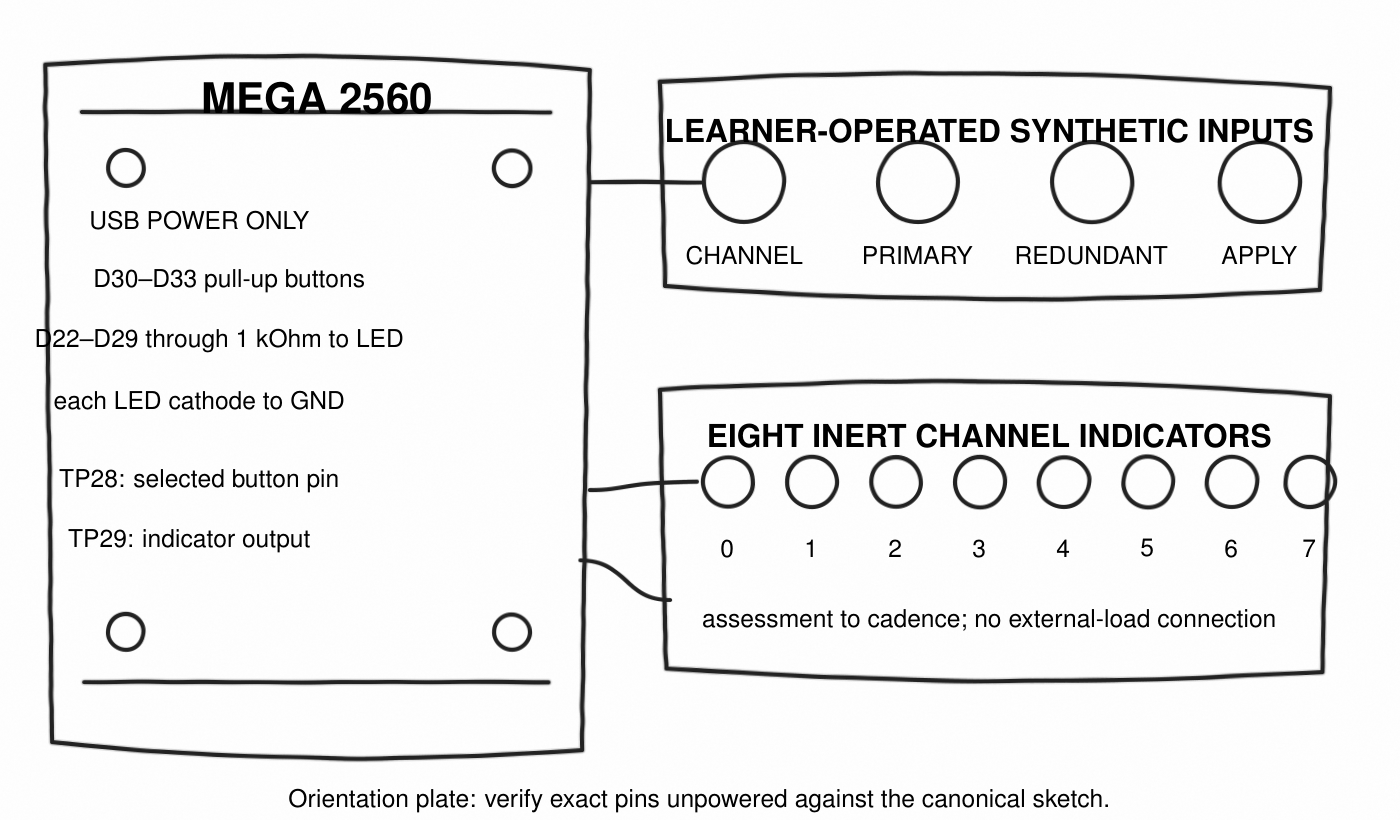
\includegraphics[width=0.96\linewidth]{028-inert-channel-pencil.png}

\small\textit{Alternative text: graphite orientation plate showing one
USB-powered Mega, four pull-up buttons on D30--D33, eight separately
resistor-limited LEDs on D22--D29, input test point TP28, and indicator test
point TP29. No external-load interface is present.}
\end{center}

\begin{tabularx}{\linewidth}{@{}l l X@{}}
\toprule
Role & Mega pin & Connection\\
\midrule
channel indicators & D22--D29 & pin to 1 k\(\Omega\), LED anode; cathode to GND\\
channel, primary, redundant, apply & D30--D33 & momentary switch to GND; internal pull-up\\
TP28 & selected input pin & meter or logic probe relative to Mega GND\\
TP29 & selected indicator pin & meter or logic probe relative to Mega GND\\
\bottomrule
\end{tabularx}

\textbf{Unpowered check.} Confirm one resistor per LED, LED polarity,
switch-to-ground wiring, and common ground. Nothing leaves the USB-powered
low-voltage teaching circuit.

\section{Truth table before code}

\begin{tabularx}{\linewidth}{@{}l l l X@{}}
\toprule
Primary & Redundant & Assessment & Why\\
\midrule
open & open & open & same usable value\\
closed & closed & closed & same usable value\\
short-simulated & short-simulated & short-simulated & same synthetic selection\\
two different usable values & --- & contradictory & evidence disagrees\\
either unavailable & any & unavailable & one required observation is absent\\
either older than threshold & any & stale & age dominates classification\\
\bottomrule
\end{tabularx}

Age equal to \texttt{staleAfter} retains the underlying state. The first
greater age is stale. The half-range timestamp rule prevents an ambiguous
future value from being mistaken for old evidence.

\section{Lifecycle and transactional update}

Construction is inert. \texttt{initialize()} rejects a zero or ambiguous stale
interval, repeated initialization is harmless, \texttt{shutdown()} is
idempotent, and destruction calls shutdown. No heap, exception, RTTI, hidden
clock, callback, or hardware owner appears in the assessor.

\texttt{update()} first validates the complete submission. It rejects:

\begin{itemize}
  \item more than eight entries or null storage with a nonzero count;
  \item an ID outside 0--7 or the same ID twice;
  \item an invalid observation enum;
  \item a timestamp in the ambiguous future half of the 32-bit space.
\end{itemize}

Only after all entries pass does it replace slots. Therefore a bad final entry
cannot partly overwrite earlier channels.

For example, if a submitted set ends with a duplicate channel, the entire set
is rejected and every preceding channel keeps its earlier assessment. An
omitted channel likewise retains its last accepted observation.

\section{Recorded evidence source}

\texttt{RecordedInertObservationSource} walks caller-owned immutable sets.
Each set holds all eight observations and one due time. Times are strictly
increasing and remain within the unambiguous 32-bit interval.

\begin{lstlisting}[style=adkcpp]
source.update   (now);
snapshot = source.snapshot ();
assessor.update (now, snapshot.observations,
                 snapshot.observationCount);
\end{lstlisting}

A delayed update selects the latest due complete set. It never emits each
missed set as a burst. Repeated snapshots expose the same pointers and values
until another set becomes due. The caller must keep the immutable storage alive
longer than the source.

For sets due at 100, 200, and 300 ms, calls at 90, 250, 250, and 400 ms expose
no set, the 200 ms set, the same 200 ms set, and the 300 ms set. The delayed
250 ms call coalesces rather than replaying the missed 100 ms set.

\section{Narrative Mega example}

\begin{lstlisting}[style=adkcpp]
observeOperator   (now);
decideAssessments (now);
showAssessments   (now);
\end{lstlisting}

Objects appear in dependency order: runtime, buttons, indicators, assessor,
then observation values. Setup acquires every owner, configures all channels
open, and starts the panel. The loop observes debounced events, decides only
when Apply submits a complete set, then presents all assessments.

At startup, one light travels across all eight indicators for two seconds.
That response proves that acquisition reached the presentation stage; it is
not a continuity claim. Channel selects 0--7. Primary and Redundant cycle
open, closed, short-simulated, unavailable. Apply timestamps and submits the
selected channel while preserving the other seven entries.

\subsection{Three dependent wins}

The short opening journey makes each new idea depend on the preceding one:

\begin{enumerate}
  \item On channel 0, submit Closed/Closed. One steady reward lamp confirms
        matching usable evidence.
  \item On channel 1, submit Open/Closed. Two reward lamps confirm that
        disagreement is distinct from either usable state.
  \item On channel 2, submit Unavailable/Closed. All eight lamps pulse for the
        final reward, confirming that missing evidence dominates disagreement.
\end{enumerate}

Submitting a later answer early produces its ordinary state cadence but does
not unlock a reward. Each reward lasts 1.5 seconds, then the panel returns to
the channel assessments. The panel always shuts down two minutes after startup,
independent of button input.

\begin{tabularx}{\linewidth}{@{}l l X@{}}
\toprule
State & Indicator & Interpretation\\
\midrule
open & off & matching open selections\\
closed & steady & matching closed selections\\
short-simulated & 1 s on / 1 s off & matching synthetic short selection\\
stale & 200 ms pulse each second & last accepted observation is too old\\
contradictory & 200 ms alternating & usable observations disagree\\
unavailable & two 120 ms pulses per 2 s & one observation unavailable\\
\bottomrule
\end{tabularx}

\section{Predict, observe, interpret}

\begin{enumerate}
  \item Predict the startup sweep, then power the panel and observe it.
  \item Complete the three ordered wins above, predicting each reward before
        Apply.
  \item After a reward clears, compare its channel cadence with the truth
        table and interpret only against the synthetic model.
  \item Stop applying. Predict and observe stale after five seconds.
  \item Leave the buttons untouched and observe every indicator release at the
        fixed two-minute ending.
\end{enumerate}

\lessonbox{\textbf{Two separate checks.} A successful startup response supports
the claim that resources were acquired. It does not prove shutdown. The fixed
ending releases every indicator; a dark LED alone is not electrical proof of
high impedance.}

\section{Diagnosis}

\begin{tabularx}{\linewidth}{@{}l X X@{}}
\toprule
Observation & Likely cause & Next bounded check\\
\midrule
no indicators ever respond & acquisition failure or wiring error & inspect D22--D29 and each resistor unpowered\\
button never changes selection & switch not reaching GND & observe TP28 high then low\\
unexpected contradictory cadence & selected values differ & cycle both banks to a known matching pair\\
all active channels become stale & no recent Apply event & apply one known pair and time five seconds\\
one LED disagrees with TP29 & LED polarity or open resistor path & compare pin level, resistor, and diode orientation\\
shutdown LED dark but pin driven & light is not high-impedance proof & measure TP29 electrically\\
\bottomrule
\end{tabularx}

\section{Go further}

After the three wins, try Short-simulated/Short-simulated and wait for it to
become stale. Then explain why a generic output callback would violate the
inert boundary even if this particular sketch connected only LEDs. The
repository's automated tests cover rejected transactions, rollover, lifecycle,
deterministic replay, compilation, and publication without turning those
release checks into learner chores.

\section{Reference trail}

\begin{itemize}
  \item \href{https://spincyc.github.io/adk/lessons/028/}
        {Searchable Lesson 028 HTML reference}
  \item \href{https://github.com/spincyc/adk/blob/main/src/inert_channel_assessor.h}
        {Public assessment and recorded-source interface}
  \item \href{https://github.com/spincyc/adk/blob/main/tests/test_inert_channel_assessor.cpp}
        {Deterministic lifecycle, transaction, timing, and replay tests}
  \item \href{https://github.com/spincyc/adk/blob/main/docs/design/LESSONS_028_030.md}
        {Lessons 028--030 safety and composition design}
  \item \href{https://docs.arduino.cc/resources/datasheets/A000067-datasheet.pdf}
        {Arduino Mega 2560 Rev3 datasheet}
\end{itemize}

\end{document}
